\documentclass{report}

\usepackage{float}
\usepackage{tikz}
\usepackage{listings}

\usetikzlibrary{shapes,
                arrows,
                decorations.pathreplacing,
                positioning,
                patterns,
                fit}

\title{Main documentation}

% Define block styles

\tikzset{block/.style=
   {rectangle,
    draw,
    text centered,
    rounded corners,
    minimum height=4em}}

\tikzset{instruction/.style =
   {rectangle split,
    rectangle split parts=5,
    rectangle split horizontal,
    draw,
    text centered,
    minimum height=2em}}

\tikzset{instruction-bits-variable/.style =
    {rectangle split,
     rectangle split
     horizontal,
     draw,
     text centered,
     minimum height=1em}}

\tikzset{instruction-bits/.style =
   {rectangle split,
    rectangle split parts=8,
    rectangle split horizontal,
    draw,
    text centered,
    minimum height=1em}}

\tikzset{arrow/.style = {draw, -latex}}

\lstdefinestyle{mainVHDL}
{
    language   = VHDL,
    frame      = single,
    breaklines = true,
    postbreak  = \mbox{\textcolor{red}{$\hookrightarrow$}\space},
    numbers    = left,
    stepnumber = 1,
    tabsize    = 4,
    captionpos = b,
    columns    = fixed
}

\newtheorem{definition}{Definition}[section]

\begin{document}

%%%%%%%%%%%%%%%%%%%%%%%%%%%%%%%%%%%%%%%%%%%%%%%%%%%%%%%%%%%%%%%%%%%%%%%%%%%%%%%%

\chapter {Background - asynchronous circuits}

There are 3 design phases in the construction of an asynchronous circuit:

\begin{itemize}
    \item Channel model specification - defines the communication channels
    between processes
    \item Handshaking protocol specification - defines the signal transitions on
    each communication channel (2-phase or 4-phase)
    \item Data encoding protocol specification - defines the data and
    handshaking assignments to wires (dual rail or bundled data)
\end{itemize}

%%%%%%%%%%%%%%%%%%%%%%%%%%%%%%%%%%%%%%%%%%%%%%%%%%%%%%%%%%%%%%%%%%%%%%%%%%%%%%%%

\section {Channel model specification}

\subsection {Definitions}

A channel exists between 2 processes. Each process connects to zero or more
channels via ports.

The channel specification is orthogonal to the handshaking specification and
the data encoding protocols used.

%%%%%%%%%%%%%%%%%%%%%%%%%%%%%%%%%%%%%%%%%%%%%%%%%%%%%%%%%%%%%%%%%%%%%%%%%%%%%%%%

\subsection {Specification}

\subsubsection {Representation}

The channel model specification can be defined in VHDL and with the aid of
channel model diagrams, as shown in Figure \ref{fig:passive-active-channels}.
Note that the arrow should point to from the process initiating the
communication.

\begin {figure}[H]
\centering
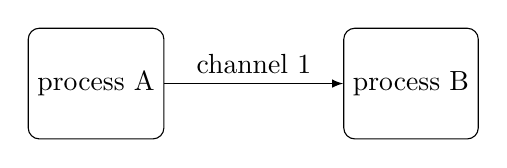
\begin{tikzpicture}[auto]

    % Place nodes
    \node [block] (processA) {process A};
    \node [block, right of=processA, node distance=4cm] (processB) {process B};

    % Draw edges
    \path [arrow]
    (processA)
    -- node [midway,above ] { channel 1}
    (processB);

\end{tikzpicture}
\caption {Channel between process A (producer) and process B (consumer).}
\label {fig:passive-active-channels}
\end {figure}

Given 2 processes, producer and consumer, and a channel between them, the VHDL
channel description is shown in Listing \ref{lst:active-passive-channel}.

\begin{lstlisting} [caption = {Channel between producer and consumer processes},
                    style   = mainVHDL,
                    label   = {lst:active-passive-channel}]
entity async_block is
end entity async_block;

architecture channel_spec of async_block is
    -- Channel
    signal ChannelProdToCons : channel := init_channel;

    -- Data units
    signal producedData : std_logic_vector(2 downto 0);
    signal consumedData : std_logic_vector(2 downto 0);
begin
    producer : process
    begin
        producedData <= selection(8, 3); -- 3 bits, 8 possibilities

        wait for delay(5, 10); -- Random delay between 5-10 units

        send(ChannelProdToCons, producedData);
    end process producer;

    consumer : process
    begin
        receive(ChannelProdToCons, consumedData);

        wait for delay(2, 5); -- Consume data
    end process consumer;
end architecture channel_spec;
\end{lstlisting}

Here the data and control signals are sent over the channel. The
\lstinline{producedData} is copied on the channel on the producer side. On the
consumer side the data from the channel is copied on the local
\lstinline{consumedData} signals.

Ideally, the consumers and producers should be defined as separate components,
as shown in Listing \ref{lst:independent-producer-consumer}.

\begin{lstlisting} [caption = {Consumer and producer are independent},
                    style   = mainVHDL,
                    label   = {lst:independent-producer-consumer}]
-- producer.vhd

entity producer is
    port(channelToConsumer : inout channel := init_channel);
end entity producer;

architecture channel_spec of producer is
    signal producedData : std_logic_vector(2 downto 0);
begin
    main : process
    begin
        producedData <= selection(8, 3);

        wait for delay(5, 10);

        send(channelToConsumer, producedData);
    end process main;
end architecture channel_spec;

-- consumer.vhd

entity consumer is
    port(channelFromProducer : inout channel := init_channel);
end entity consumer;

architecture channel_spec of consumer is
    signal consumedData : std_logic_vector(2 downto 0);
begin
    main : process
    begin
        receive(channelFromProducer, consumedData);

        wait for delay(2, 5);
    end process main;
end architecture channel_spec;
\end{lstlisting}

%%%%%%%%%%%%%%%%%%%%%%%%%%%%%%%%%%%%%%%%%%%%%%%%%%%%%%%%%%%%%%%%%%%%%%%%%%%%%%%%

\subsubsection{Deadlocks}

A port can be either active or passive.

The process with the active port initiates the communication (handshaking) while
the process with the passive port waits for an initiation.

For valid communication (without deadlocks) to occur, a channel shall be
connected to a passive port on one end and an active port on the other end.

Deadlocks may occur when processes handle multiple channels. While waiting to
receive data on one channel, the other process is trying to send data on another
channel, as shown in Listing \ref{lst:deadlock-example}.

\begin {figure}[H]
\centering
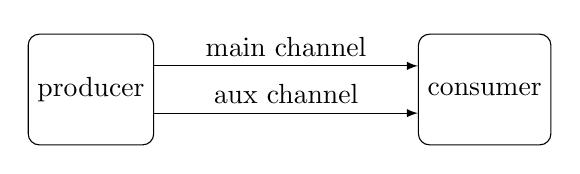
\begin{tikzpicture}[auto]

    % Place nodes
    \node [block] (processA) {producer};
    \node [block, right of=processA, node distance=5cm] (processB) {consumer};

    % Draw edges
    \path [arrow]
    ([yshift = 0.3cm] processA.east)
    -- node [midway,above] { main channel }
    ([yshift = 0.3cm] processB.west);

    \path [arrow]
    ([yshift = -0.3cm] processA.east)
    -- node [midway,above] { aux channel}
    ([yshift = -0.3cm] processB.west);

\end{tikzpicture}
\caption {Multiple channels between a consumer and producer.}
\label {fig:multiple-channels}
\end {figure}

\begin{lstlisting} [caption = {Deadlock example},
                    style   = mainVHDL,
                    label   = {lst:deadlock-example}]
producer : process
begin
    wait for delay(5, 10);
    send(mainChannelToConsumer, mainProducedData);

    wait for delay(5, 10);
    send(auxChannelToConsumer, auxProducedData);
end process main;

consumer : process
begin
    receive(auxChannelFromProducer, auxConsumedData); -- Deadlock
    receive(mainChannelFromProducer, mainConsumedData);

    wait for delay(2, 5);
end process main;
\end{lstlisting}

The producer tries to send data on the main channel while the consumer is
waiting for data on the aux channel.

\textbf{Note:} To prevent deadlocks, the consumer has to first probe the
channels to check if they have data on them. Only then the consumer may receive
data on those channels, as shown in Listing \ref{lst:channel-probing}. This is
not required when a single channel is used between the consumer and producer.

\begin{lstlisting} [caption = {Channel probing},
                    style   = mainVHDL,
                    label   = {lst:channel-probing}]
producer : process
begin
    wait for delay(5, 10);
    send(mainChannelToConsumer, mainProducedData);

    wait for delay(5, 10);
    send(auxChannelToConsumer, auxProducedData);
end process main;

consumer : process
begin
    if (probe(auxChannelFromProducer)) then
        receive(auxChannelFromProducer, auxConsumedData);
    elsif (probe(mainChannelFromProducer)) then
        receive(mainChannelFromProducer, mainConsumedData);
    end if;

    wait for delay(2, 5);
end process main;
\end{lstlisting}

\textbf{Note:} The process which probes a channel should, therefore, be
connected to the passive end of that channel.

%%%%%%%%%%%%%%%%%%%%%%%%%%%%%%%%%%%%%%%%%%%%%%%%%%%%%%%%%%%%%%%%%%%%%%%%%%%%%%%%

\section{Sequential communication}

\subsection{Single channel communication}

Given a single channel between a consumer and a producer, a single unit of data
is communicated at a time. The producer creates a data unit and sends it over
the channel as shown in Listing \ref{lst:single-channel-producer}.

\begin{lstlisting} [caption = {Single channel producer},
                    style   = mainVHDL,
                    label   = {lst:single-channel-producer}]
producer : process
begin
    wait for delay(5, 10);

    send(mainChannel, data);
end process producer;
\end{lstlisting}

The consumer  then receives the data unit as shown in Listing
\ref{lst:single-channel-consumer}.

\begin{lstlisting} [caption = {Single channel consumer},
                    style   = mainVHDL,
                    label   = {lst:single-channel-consumer}]
consumer : process
begin
    receive(mainChannel, data);

    wait for delay(5, 10);
end process consumer;

\end{lstlisting}

This is the simplest way to communicate as it only requires a single channel.
This also expands into a small and simple circuit. The performance however,
is sacrificed as no data can be communicated in parallel.

The resulting connections between the processes is simple as a process
communicates with exactly one other process. Also no deadlocks can occur.

\begin{table}[H]
    \centering
    \begin{tabular}{ r c l }
        process interconnect & $\rightarrow$ & simple \\
        data flow            & $\rightarrow$ & simple \\
        performance          & $\rightarrow$ & low \\
        circuit size         & $\rightarrow$ & small \\
        deadlock chance      & $\rightarrow$ & not possible \\
    \end{tabular}
\end{table}

%%%%%%%%%%%%%%%%%%%%%%%%%%%%%%%%%%%%%%%%%%%%%%%%%%%%%%%%%%%%%%%%%%%%%%%%%%%%%%%%

\subsection{Multiple channel sequential communication}

Given multiple channels connected to a consumer or a producer, a single unit of
data is communicated over a single channel at a time.

This type of communication requires a producer to be connected to multiple
consumers and vice versa as shown in Figure
\ref{fig:multi-channel-communication}. The producer can only produce one data
unit at a time.

\begin {figure}[H]
\centering
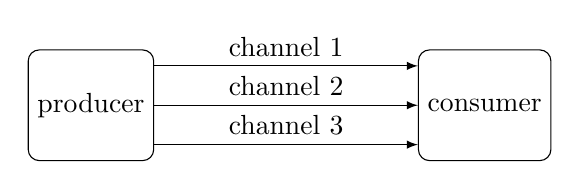
\begin{tikzpicture}[auto]

    % Place nodes
    \node [block] (producer) {producer};
    \node [block, right of=producer, node distance=5cm] (consumer) {consumer};

    % Draw edges
    \path [arrow]
    ([yshift = 0.5cm] producer.east)
    -- node [midway,above] { channel 1 }
    ([yshift = 0.5cm] consumer.west);

    \path [arrow]
    (producer.east)
    -- node [midway,above] { channel 2 }
    (consumer.west);

    \path [arrow]
    ([yshift = -0.5cm] producer.east)
    -- node [midway,above] { channel 3}
    ([yshift = -0.5cm] consumer.west);

\end{tikzpicture}
\caption {Sequential communication over multiple channels.}
\label {fig:multi-channel-communication}
\end {figure}

The resulting connections between processes is complex as a single process
communicates with multiple processes.

\begin{table}[H]
    \centering
    \begin{tabular}{ r c l }
        process interconnect & $\rightarrow$ & complex \\
        data flow            & $\rightarrow$ & simple \\
        performance          & $\rightarrow$ & low \\
        circuit size         & $\rightarrow$ & large \\
        deadlock chance      & $\rightarrow$ & possible unless probing is used \\
    \end{tabular}
\end{table}

\subsubsection{Producer}

The producer creates a data unit and places it on a channel. It then creates
another data unit and places it on another channel (which may be the same as the
previous channel). The producer makes the choice of what data to send over which
channel at any time. No data is communicated in parallel.

As shown in Listing \ref{lst:multi-channel-producer}, the producer sends data
over the second channel, then over the first channel and lastly over the third
channel before restarting the flow.

\begin{lstlisting} [caption = {Multiple channel producer},
                    style   = mainVHDL,
                    label   = {lst:multi-channel-producer}]
consumer : process
begin
    data <= selection(8, 3);
    wait for delay(5, 10);
    send(channel2, data);

    data <= selection(8, 3);
    wait for delay(5, 10);
    send(channel1, data);

    data <= selection(8, 3);
    wait for delay(5, 10);
    send(channel3, data);
end process consumer;

\end{lstlisting}

\subsubsection{Consumer}

The consumer has to check which of the channels has data and then wait to
receive the data from that channel. The consumer makes the choice in which order
to check which channels have data.

The consumer has to also probe the channels to prevent deadlocks as shown in
Listing \ref{lst:multi-channel-consumer-probing}.

\begin{lstlisting} [caption = {Multiple channel consumer with probing},
                    style   = mainVHDL,
                    label   = {lst:multi-channel-consumer-probing}]
consumer : process
begin
    if (probe(channel1)) then
        receive(channel1, data);
    elsif (probe(channel2)) then
        receive(channel2, data);
    elsif (probe(channel3)) then
        receive(channel3, data);
    end if;

    wait for delay(5, 10);
end process consumer;

\end{lstlisting}

If there is a strict protocol which decides which channel to use next and both,
the producer and consumer adhere to it, probing may be skipped as shown in
Listing \ref{lst:multi-channel-consumer-no-probing}.

\begin{lstlisting} [caption = {Multiple channel consumer without probing},
                    style   = mainVHDL,
                    label   = {lst:multi-channel-consumer-no-probing}]
consumer : process
begin
    receive(channel2, data);
    wait for delay(5, 10);

    receive(channel1, data);
    wait for delay(5, 10);

    receive(channel3, data);
    wait for delay(5, 10);
end process consumer;

\end{lstlisting}

%%%%%%%%%%%%%%%%%%%%%%%%%%%%%%%%%%%%%%%%%%%%%%%%%%%%%%%%%%%%%%%%%%%%%%%%%%%%%%%%

\section{Multiple channel parallel communication}

Given multiple channels connected to a producer or a consumer, multiple data
units are communicated over multiple channels at any time.

This is the most complex type of communication as an arbitrary number of data
units can be communicated over an arbitrary number of channels at any time.

\begin{definition}{\textbf{Parallel transaction}}
    A set of data units sent over a multiple channels at once.
\end{definition}

Note that the set of data may be sent in parallel to multiple consumers.
Different parts of the parallel transaction may correspond to different
consumers.

\begin{table}[H]
    \centering
    \begin{tabular}{ r c l }
        process interconnect & $\rightarrow$ & complex \\
        data flow            & $\rightarrow$ & complex \\
        performance          & $\rightarrow$ & high \\
        circuit size         & $\rightarrow$ & large \\
        deadlock chance      & $\rightarrow$ & possible unless probing is used \\
    \end{tabular}
\end{table}

\subsection{Producer}

\subsubsection{Strongly indicating parallel communication}

The producer creates N data units and sends them over N channels. After all N
data units have been sent it then creates M data units and sends them over M
channels. N may or may not be the same as M. This allows the producer to
communicate some data on multiple channels at once.

The producer sends all the data units at any time all at once and will only send
more data units once the previous units have been successfully received by the
consumer as shown in Listing \ref{lst:strong-parallel-producer}. The producer
send data over channels 0 and 1 in parallel. It then waits for the transaction
to finish before sending data over channels 2 and 0 in parallel.

It is called strongly indicating as the producer has to wait for all the sent
data to be fully consumed before it can send any further data on possibly other
channels.

\begin{lstlisting} [caption = {Strongly indicating parallel channel producer},
                    style   = mainVHDL,
                    label   = {lst:strong-parallel-producer}]
producer : process
begin
    wait for delay(5, 10);
    send(channel0, data0,
         channel1, data1);

    wait for delay(5, 10);
    send(channel2, data2,
         channel0, data0);
end process consumer;
\end{lstlisting}

\subsubsection{Weakly indicating parallel communication}

The producer may wish to start sending data early if enough but not all data has
been consumed. For instance the producer may send data units on the first 3
channels in parallel. If the data on channels 0 and 1 have been consumed early,
the producer can send more data on channels 0, 1 and possibly other channels but
not channel 2. It is called weakly indicating as only a part of the complex
transaction needs to be completed before the next transaction may start.

Good designs should not lead to this type of producer as it hides too many
details to be fully specified in VHDL. For instance, the send procedure should
terminate before continuing. Instead multiple strongly indicating producer
processes should be devised.

\subsection{Consumer}

The consumer may naively just probe each channel and receive data on the
channels with available data. To fully exploit the parallelism advantages, the
consumer should know at any time which producer is sending parallel data on
which channels and them receive that data in parallel. In such case, the
consumer should skip probing and begin receiving data on those channels, as
shown in Listing \ref{lst:parallel-consumer}.

\begin{lstlisting} [caption = {Parallel channel consumer},
                    style   = mainVHDL,
                    label   = {lst:parallel-consumer}]
consumer : process
begin
    receive(channel0, data0,
            channel1, data1);
    wait for delay(5, 10);

    receive(channel2, data2,
            channel0, data0);
    wait for delay(5, 10);
end process consumer;
\end{lstlisting}

\section{Multistage data flow}

Thus far only single stage data flows have been discussed. A data flow is the
aggregate number of channels between 2 processes, forming a single stage. The
channels between the second and the next process form a second data flow stage,
as shown in Figure \ref{fig:multistage-dataflow}.

\begin {figure}[H]
\centering
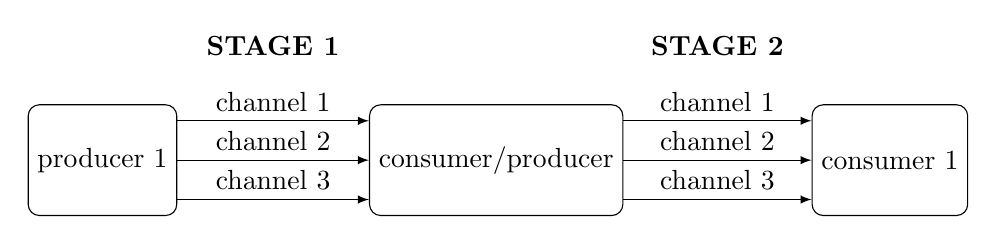
\begin{tikzpicture}[auto]

    % Blocks
    \node [block] (producer1) {producer 1};
    \node [block, right of=producer1, node distance=5cm] (consumer1) {consumer/producer};
    \node [block, right of=consumer1, node distance=5cm] (producer2) {consumer 1};

    % Draw edges
    % Stage 1
    \path [arrow]
    ([yshift = 0.5cm] producer1.east)
    -- node [midway,above] { channel 1 }
    ([yshift = 0.5cm] consumer1.west);

    \path [arrow]
    (producer1.east)
    -- node [midway,above] { channel 2 }
    (consumer1.west);

    \path [arrow]
    ([yshift = -0.5cm] producer1.east)
    -- node [midway,above] { channel 3}
    ([yshift = -0.5cm] consumer1.west);

    % Stage 2
    \path [arrow]
    ([yshift = 0.5cm] consumer1.east)
    -- node [midway,above] { channel 1 }
    ([yshift = 0.5cm] producer2.west);

    \path [arrow]
    (consumer1.east)
    -- node [midway,above] { channel 2 }
    (producer2.west);

    \path [arrow]
    ([yshift = -0.5cm] consumer1.east)
    -- node [midway,above] { channel 3}
    ([yshift = -0.5cm] producer2.west);

    % Stages
    \path
    ([yshift = 1.2cm] producer1.east)
    -- node [midway,above] { \textbf{STAGE 1}}
    ([yshift = 1.2cm] consumer1.west);

    \path
    ([yshift = 1.2cm] consumer1.east)
    -- node [midway,above] { \textbf{STAGE 2}}
    ([yshift = 1.2cm] producer2.west);

\end{tikzpicture}
\caption {Double stage data flow.}
\label {fig:multistage-dataflow}
\end {figure}

\section{Process specification}

A process has the following elements:

\begin{itemize}
    \item{Type: producer, consumer or both}
    \item{State: internal signals which are possibly read and set for each
        input}
    \item{Logic: a logic or arithmetic (or both) block which operates on the
        input signals and the internal signals, much like a state machine}
\end{itemize}

Start point and end point processes are either producers or consumers but not
both. Usually a process behaves like a state machine, transforming the input
signals and internal signals into output signals.

\section{Complete specification}

There may be a hierarchy of static and dynamic block diagrams. Blocks in the
upper levels of the hierarchy contain a subset of blocks from a lower level in
the hierarchy.

The channel model diagrams and specifications are only done for the blocks at
the lowest level in the hierarchy as only at that level there is sufficient
detail.

\subsection{Diagrams}

\subsubsection{Static diagrams}

A block diagram describes the main processes and the main data flow between
them.
A channel diagram describes all processes and all the channels between them.

\subsubsection{Dynamic diagrams}

These also include block and channel diagrams, however, rather than only showing
the channels between the processes, they also describe which channels and which
processes are used for specific inputs (such as instructions, control signals,
etc.).

\subsection{Specifications}

A channel model specification describes (using VHDL) the connection between all
processes (represented as components in VHDL) based on the static channel
diagram.

The process specification describes (using VHDL) each process' elements based on
the dynamic channel diagram.

\chapter{Processor architecture}

\section{Background}

The dataflow through a processor consists of 3 stages, as shown in Figure
\ref{fig:processor-dataflow-stages}:

\begin{itemize}

\item Data and instruction fetch
\item Instruction decoding
\item Instruction execution

\end{itemize}

\begin {figure}[H]
\centering
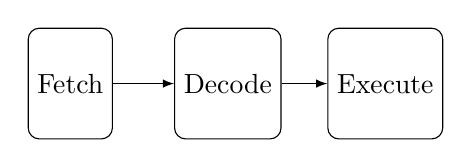
\begin{tikzpicture}[auto]

    % Blocks
    \node [block] (fetch) {Fetch};
    \node [block, right of=fetch, node distance=2cm] (decode) {Decode};
    \node [block, right of=decode, node distance=2cm] (execute) {Execute};

    % Draw edges

    \path [arrow]
    (fetch.east) -- (decode.west);

    \path [arrow]
    (decode.east) -- (execute.west);

\end{tikzpicture}
\caption {Processor dataflow stages}
\label {fig:processor-dataflow-stages}
\end {figure}


%%%%%%%%%%%%%%%%%%%%%%%%%%%%%%%%%%%%%%%%%%%%%%%%%%%%%%%%%%%%%%%%%%%%%%%%%%%%%%%%

\section{Fetch: Caching}

\subsection{Background}

The instructions and data are stored in the primary memory (usually RAM), which
are then fetched and executed by the processor. Usually the processor executes
an instruction faster than it is fetched, thus the primary memory stalls the
processor execution.

The cache is a small and fast memory block located around or inside the
processor. It holds a small portion of the primary memory, specifically around
the current instruction or data pointers. This was the processor can access
the instructions and data at the cache speed rather than the primary memory
speed, thus improving execution speed. The cache inside the processor usually
operates at the same speed as the processor and thus the execution is not
stalled. The cache around the processor is larger but slightly slower than the
cache inside the processor.

\subsection{Cache layout}

There are 3 levels of cache:

\begin{itemize}
    \item { Level 1 (L1) - cache is located inside each of the processor's cores. It
        operates at the core speed and is rather small.}

    \item { Level 2 (L2) - cache is located inside the processor and is shared among
        the processor's cores. It is slower than L1 cache but larger.}

    \item { Level 3 (L3) - cache is located around the processor. It is slower
        than L2 but larger.  }

\end{itemize}

The cache may follow a unified architecture, thus holding both instructions and
data, or split holding instructions and data in separate sections. The later
allows for parallel cache accesses.

The primary memory stored data in blocks.

The cache stores data in cache lines.

The processor registers store data in words.

A cache can be described in terms of the number of cache lines and the cache
line width. Each cache line contains 3 elements, the cache data, a tag and a set
of control/valid bits.

Let $size(c)$ be the number of cache lines in cache $c$.

Let $width(c)$ be the width of a cache line in cache $c$.

Let $width_{tag}(c)$ be the width of the tag field in a cache line of cache $c$.

Let $width_{data}(c)$ be the width of the data field in a cache line of cache
$c$.

Let $width_{control}(c)$ be the width of the control/valid bits field in a cache
line of cache $c$.

Let $tag_c(n)$ be the tag value of cache line $n$ of cache $c$.

Let $data_c(n)$ be the data value of cache line $n$ of cache $c$.

Let $control_c(n)$ be the value of the control/valid field of cache line $n$ of
cache $c$.

\subsection{Cache mapping}

Cache mapping refers to which cache lines can hold which primary memory blocks.

When a cache becomes full, a cache line replacement algorithm is used to decide
which cache lines to replace.

\subsubsection{Direct mapping}

A block of the main memory maps only to a single cache line.

The cache line number is given by:

\begin{equation}
    N = A \bmod size(c)
\end{equation}

where $A$ is the primary memory address and $N$ is the mapped cache line number.

When the cache becomes full, the cache line mapped to the new memory fetch is
replaced. The replacement algorithm is a simple direct memory assignment.

This type of mapping is rather effective when the entire primary memory is used
evenly. If one part of the primary memory is used more often, and some parts of
the primary memory are not used at all, some cache lines may not be used at all,
thus reducing the amount of effective cache.

The tag and some of the control bits represent the block number.

\subsubsection{Fully associative mapping}

Any cache line can be mapped to any memory location. This mapping requires a
more elaborate cache replacement algorithm.

\subsubsection{Set associative mapping}

The cache is divided into sets of cache lines. Each set can only map to a single
part of the primary memory. Within each set, the cache lines can map to any
block of memory.

Essentially, there is direct mapping at the set level and fully associative
mapping at the cache line level within a set.

The number of cache lines in a set is known as the $k$ value, hence the mapping
is described as $k$-way set associative mapping.

Direct mapping therefore is 1-way associative mapping.

\subsection{Cache write strategies}

\subsubsection{Write-through}

The primary memory is updated immediately once the cache is updated. This often
creates excessive primary memory traffic.

\subsubsection{Write-back}

The primary memory is only updated when a cache line is replaced. This posses
some risk when the primary memory is used by other peripherals as well as it may
not hold the most up-to-date contents.

\subsection{Cache replacement strategies}

Spacial locality refers to the likelihood of the next memory fetches to be
around the current instruction or data pointers.

Temporal locality refers to the likelihood of the same memory fetches to be done
again in the near future.

Different caching strategies are used to improve spacial and temporal
localities.

When the value of a memory fetch is available in cache, the processor has
\textbf{hit the cache}. Similarly, when the value of the memory fetch is not
available in cache, the processor has \textbf{missed the cache}.

Note: When the cache of each core hold a copy of the same cache line, it is
enough for one core to update the value of the cache line to render the same
cache line invalid on the other cores. The cache is said to be coherent when it
marks the cache line as invalid when such event occurs.

It is more problematic however on multiprocessor systems, where there is a
rather high latency between the data becoming incoherent and it being marked as
invalid.


%%%%%%%%%%%%%%%%%%%%%%%%%%%%%%%%%%%%%%%%%%%%%%%%%%%%%%%%%%%%%%%%%%%%%%%%%%%%%%%%

\section{Decode: Instruction set architecture}

The job of a processor is to execute a stream of instructions. The supported
instructions definitions and descriptions form an instruction set.


%%%%%%%%%%%%%%%%%%%%%%%%%%%%%%%%%%%%%%%%%%%%%%%%%%%%%%%%%%%%%%%%%%%%%%%%%%%%%%%%

\subsection{Instruction format}

The instruction format describes the components of an instruction and their
location within it as shown in Figure \ref{fig:instruction-format-components}.

\begin {figure}[H]
\centering
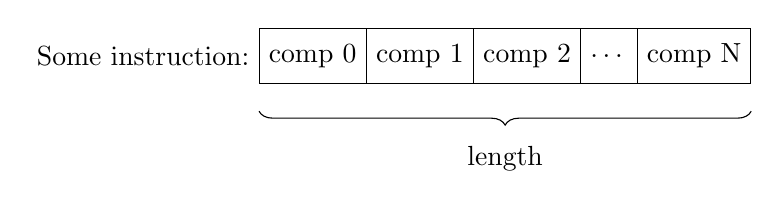
\begin{tikzpicture}[auto]

    \node [instruction, label=west:{Some instruction:}] (main)
    {\nodepart{one}   {comp 0}
     \nodepart{two}   {comp 1}
     \nodepart{three} {comp 2}
     \nodepart{four}  {\ldots}
     \nodepart{five}  {comp N}};

    \draw [decorate, decoration={brace, mirror, amplitude=0.5em}]
     ([yshift=-2em]main.west) -- ([yshift=-2em]main.east)
     node [black,midway,yshift=-2.5em] {length};

\end{tikzpicture}
\caption {Instruction format components}
\label {fig:instruction-format-components}
\end {figure}

\subsubsection{Length}

\begin{itemize}
    \item{Fixed length - all instructions are of equal length as shown in Figure
        \ref{fig:fixed-instruction-length}. All instructions in memory are
        aligned as shown in Figure \ref{fig:aligned-fixed-instruction-length}.
        This type of instructions take more memory, however they can be decoded
        faster than variable length instructions as an entire instruction can
        be fed into the decoder at once.}

    \begin {figure}[H]
    \centering
    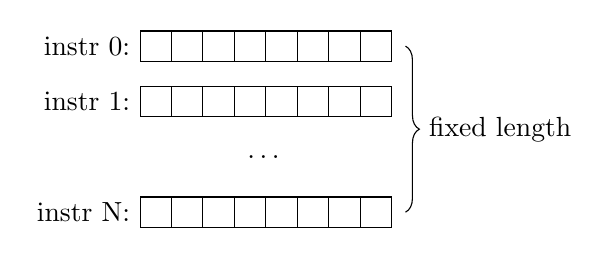
\begin{tikzpicture}[auto]

        \node [instruction-bits,
               label=west:{instr 0:}] (instr0) {};

        \node [instruction-bits,
               below of = instr0,
               node distance = 2em,
               label=west:{instr 1:}] (instr1) {};

        \node [auto=false,
               below of=instr1,
               node distance = 2em] (dots) {\ldots};

        \node [instruction-bits,
               below of = dots,
               node distance = 2em,
               label=west:{instr N:}] (instrN) {};

        \draw [decorate, decoration={brace, amplitude=0.5em}]
         ([xshift=0.5em]instr0.east) -- ([xshift=0.5em]instrN.east)
         node [black,midway, xshift=0.5em] {fixed length};

    \end{tikzpicture}
    \caption {Fixed length instructions}
    \label {fig:fixed-instruction-length}
    \end {figure}


    \item{Variable length - instructions may have different lengths as shown in
        Figure \ref{fig:variable-instruction-length}. There are
        no gaps between shorter and longer instructions and thus the
        instructions are not aligned as shown in Figure
        \ref{fig:misaligned-variable-instruction-length}. These instructions
        take less memory, however are slower to decode than fixed length
        instructions as the instruction length is not preemptively known.}
\end{itemize}

\begin {figure}[H]
\centering
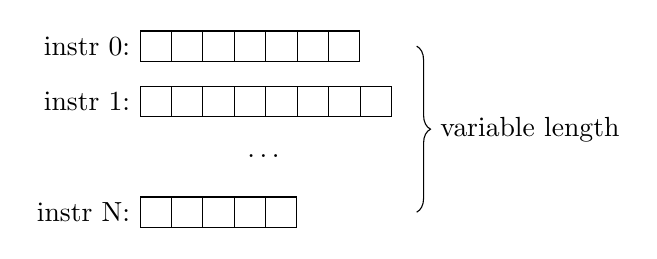
\begin{tikzpicture}[auto]

    \node [instruction-bits-variable,
           rectangle split parts=7,
           label={west:{instr 0:}}] (instr0) {};

    \node [instruction-bits-variable,
           rectangle split parts=8,
           node distance = 2em,
           label={west:{instr 1:}},
           below = of instr0.west,
           anchor=west] (instr1) {};

    \node [auto=false,
           node distance = 1em,
           below = of instr1] (dots) {\ldots};

    \node [instruction-bits-variable,
           rectangle split parts=5,
           node distance = 4em,
           label={west:{instr N:}},
           below = of instr1.west,
           anchor=west] (instrN) {};

    \draw [decorate, decoration={brace, amplitude=0.5em}]
     ([xshift=10em]instr0.west) -- ([xshift=10em]instrN.west)
     node [black,midway, xshift=0.5em] {variable length};

\end{tikzpicture}
\caption {Variable length instructions}
\label {fig:variable-instruction-length}
\end {figure}


\begin {figure}[H]
\centering
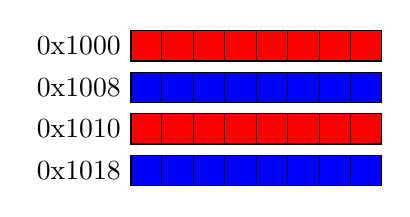
\begin{tikzpicture}[auto]

    \node [instruction-bits,
           rectangle split part fill={red},
           label=west:{0x1000}] (block0) {};

    \node [instruction-bits,
           rectangle split part fill={blue},
           below of = block0,
           node distance = 1.5em,
           label=west:{0x1008}] (block1) {};

    \node [instruction-bits,
           rectangle split part fill={red},
           below of = block1,
           node distance = 1.5em,
           label=west:{0x1010}] (block2) {};

    \node [instruction-bits,
           rectangle split part fill={blue},
           below of = block2,
           node distance = 1.5em,
           label=west:{0x1018}] (block3) {};

\end{tikzpicture}
\caption {Aligned memory with fixed length instructions}
\label {fig:aligned-fixed-instruction-length}
\end {figure}


\begin {figure}[H]
\centering
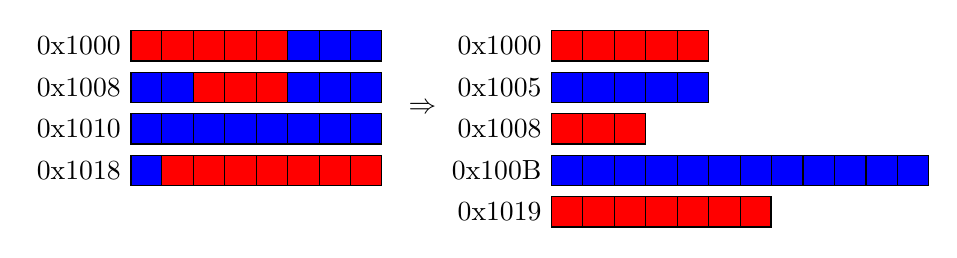
\begin{tikzpicture}[auto]

    \node [instruction-bits,
           rectangle split part fill={red, red, red, red, red, blue},
           label=west:{0x1000}] (block0) {};

    \node [instruction-bits,
           rectangle split part fill={blue, blue, red, red, red, blue},
           below of = block0,
           node distance = 1.5em,
           label=west:{0x1008}] (block1) {};

    \node [instruction-bits,
           rectangle split part fill={blue},
           below of = block1,
           node distance = 1.5em,
           label=west:{0x1010}] (block2) {};

    \node [instruction-bits,
           rectangle split part fill={blue, red},
           below of = block2,
           node distance = 1.5em,
           label=west:{0x1018}] (block3) {};

    \node [auto=false,
           xshift=6em,
           yshift = -2.25em] (arrow) {$\Rightarrow$};

    \node [instruction-bits-variable,
           rectangle split parts = 5,
           rectangle split part fill={red},
           xshift=13.5em,
           label=west:{0x1000}] (rblock0) {};

    \node [instruction-bits-variable,
           rectangle split parts = 5,
           rectangle split part fill={blue},
           node distance = 1.5em,
           label=west:{0x1005},
           below = of rblock0.west,
           anchor=west] (rblock1) {};

    \node [instruction-bits-variable,
           rectangle split parts = 3,
           rectangle split part fill={red},
           node distance = 1.5em,
           label=west:{0x1008},
           below = of rblock1.west,
           anchor=west] (rblock2) {};

    \node [instruction-bits-variable,
           rectangle split parts = 12,
           rectangle split part fill={blue},
           node distance = 1.5em,
           label=west:{0x100B},
           below = of rblock2.west,
           anchor=west] (rblock3) {};

    \node [instruction-bits-variable,
           rectangle split parts = 7,
           rectangle split part fill={red},
           node distance = 1.5em,
           label=west:{0x1019},
           below = of rblock3.west,
           anchor=west] (rblock4) {};

\end{tikzpicture}
\caption {Misaligned memory with variable length instructions}
\label {fig:misaligned-variable-instruction-length}
\end {figure}



\subsubsection{Structure}

\begin{itemize}
    \item{Fixed structure - all instructions have the same components at the
        same locations. For variable length instructions, some of the components
        may be disabled and thus not included in the instruction as shown in
        Figure \ref{fig:variable-length-fixed-structure-instructions}.
        Similarly, for fixed length instructions, some components may be
        disabled, however they are included in the instruction and are ignored
        by the decoder as shown in Figure
        \ref{fig:fixed-length-fixed-structure-instructions}. If an instruction
        is fixed length and fixed structure, it can be fed into the decoder at
        once with all of its components decoded in parallel.}
    \item{Variable structure - the instruction is decoded serially and the
        remainder of the instruction structure depends on the previous and
        current components, and even on the values of some registers. Usually
        the first component of this type of instructions is the same for all
        instructions as it is usually used to identify the instruction type.
        Also, this type of instructions are usually variable length as it is
        rather difficult and inefficient to have fixed length instructions with
        different components across the instruction set. Usually the structure
        of an instruction can be fixed yet complex, such that for variable
        length instructions there may be a large number of components, most of
        which are disabled for most instructions. This is not to be confused
        with variable structure instructions as decoding these instructions
        requires looking up the next allowed components through a tree, whereas
        fixed structure instructions have a linear lookup (with components in
        the line simply being skipped). The instructions from Figure
        \ref{fig:variable-length-variable-structure-instructions} would require
        3 branches in the lookup tree.}
\end{itemize}

Note that fixed structure instructions are are a mere subset of variable
structure instructions. The branches of the lookup tree can also merge and be
cyclic. At each divergence in the tree, the current and previous components and
some registers decide which path to take. Such instructions may be incredibly
complex and are very slow to decode.

\begin {figure}[H]
\centering
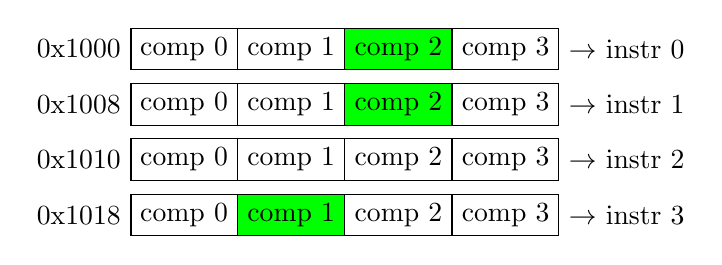
\begin{tikzpicture}[auto]

    \node [instruction-bits-variable,
           rectangle split parts = 4,
           rectangle split part fill = {white, white, green, white},
           label=east:{$\rightarrow$ instr 0},
           label=west:{0x1000}] (block0)
    {\nodepart{one}   {comp 0}
     \nodepart{two}   {comp 1}
     \nodepart{three} {comp 2}
     \nodepart{four}  {comp 3}};

    \node [instruction-bits-variable,
           rectangle split parts = 4,
           rectangle split part fill = {white, white, green, white},
           label=east:{$\rightarrow$ instr 1},
           label=west:{0x1008},
           node distance = 2em,
           below = of block0.west,
           anchor=west] (block1)
    {\nodepart{one}   {comp 0}
     \nodepart{two}   {comp 1}
     \nodepart{three} {comp 2}
     \nodepart{four}  {comp 3}};

    \node [instruction-bits-variable,
           rectangle split parts = 4,
           label=east:{$\rightarrow$ instr 2},
           label=west:{0x1010},
           node distance = 2em,
           below = of block1.west,
           anchor=west] (block2)
    {\nodepart{one}   {comp 0}
     \nodepart{two}   {comp 1}
     \nodepart{three} {comp 2}
     \nodepart{four}  {comp 3}};

    \node [instruction-bits-variable,
           rectangle split parts = 4,
           rectangle split part fill = {white, green, white, white},
           label=east:{$\rightarrow$ instr 3},
           label=west:{0x1018},
           node distance = 2em,
           below = of block2.west,
           anchor=west] (block3)
    {\nodepart{one}   {comp 0}
     \nodepart{two}   {comp 1}
     \nodepart{three} {comp 2}
     \nodepart{four}  {comp 3}};

\end{tikzpicture}
\caption {Instructions with a fixed structure (4 components) and fixed length.
          The coloured components are ignored by the decoder. Each component may
          have different lengths.}
\label {fig:fixed-length-fixed-structure-instructions}
\end {figure}


\begin {figure}[H]
\centering
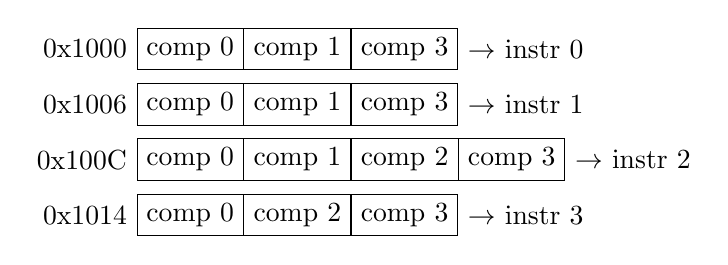
\begin{tikzpicture}[auto]

    \node [instruction-bits-variable,
           rectangle split parts = 3,
           label=east:{$\rightarrow$ instr 0},
           label=west:{0x1000}] (block0)
    {\nodepart{one}   {comp 0}
     \nodepart{two}   {comp 1}
     \nodepart{three}  {comp 3}};

    \node [instruction-bits-variable,
           rectangle split parts = 3,
           label=east:{$\rightarrow$ instr 1},
           label=west:{0x1006},
           node distance = 2em,
           below = of block0.west,
           anchor=west] (block1)
    {\nodepart{one}   {comp 0}
     \nodepart{two}   {comp 1}
     \nodepart{three}  {comp 3}};

    \node [instruction-bits-variable,
           rectangle split parts = 4,
           label=east:{$\rightarrow$ instr 2},
           label=west:{0x100C},
           node distance = 2em,
           below = of block1.west,
           anchor=west] (block2)
    {\nodepart{one}   {comp 0}
     \nodepart{two}   {comp 1}
     \nodepart{three} {comp 2}
     \nodepart{four}  {comp 3}};

    \node [instruction-bits-variable,
           rectangle split parts = 3,
           label=east:{$\rightarrow$ instr 3},
           label=west:{0x1014},
           node distance = 2em,
           below = of block2.west,
           anchor=west] (block3)
    {\nodepart{one} {comp 0}
     \nodepart{two} {comp 2}
     \nodepart{three} {comp 3}};

\end{tikzpicture}
\caption {Instructions with a fixed structure (4 components) and variable
          length. The missing components are not included in the instruction.
          Also, each component may have different lengths.}
\label {fig:variable-length-fixed-structure-instructions}
\end {figure}


\begin {figure}[H]
\centering
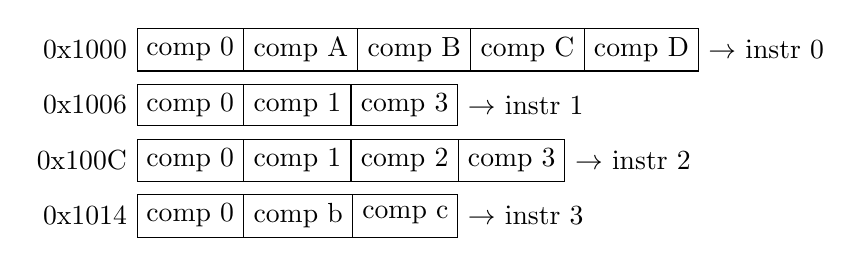
\begin{tikzpicture}[auto]

    \node [instruction-bits-variable,
           rectangle split parts = 5,
           label=east:{$\rightarrow$ instr 0},
           label=west:{0x1000}] (block0)
    {\nodepart{one}   {comp 0}
     \nodepart{two}   {comp A}
     \nodepart{three} {comp B}
     \nodepart{four}  {comp C}
     \nodepart{five}  {comp D}};

    \node [instruction-bits-variable,
           rectangle split parts = 3,
           label=east:{$\rightarrow$ instr 1},
           label=west:{0x1006},
           node distance = 2em,
           below = of block0.west,
           anchor=west] (block1)
    {\nodepart{one}   {comp 0}
     \nodepart{two}   {comp 1}
     \nodepart{three} {comp 3}};

    \node [instruction-bits-variable,
           rectangle split parts = 4,
           label=east:{$\rightarrow$ instr 2},
           label=west:{0x100C},
           node distance = 2em,
           below = of block1.west,
           anchor=west] (block2)
    {\nodepart{one}   {comp 0}
     \nodepart{two}   {comp 1}
     \nodepart{three} {comp 2}
     \nodepart{four}  {comp 3}};

    \node [instruction-bits-variable,
           rectangle split parts = 3,
           label=east:{$\rightarrow$ instr 3},
           label=west:{0x1014},
           node distance = 2em,
           below = of block2.west,
           anchor=west] (block3)
    {\nodepart{one}   {comp 0}
     \nodepart{two}   {comp b}
     \nodepart{three} {comp c}};

\end{tikzpicture}
\caption {Instructions with a variable structure (3 sets of variations, lower
          case letters, upper case letters and digits) and variable length
          (there may be gaps between the numbering or lettering). Each
          component may have different lengths.}
\label {fig:variable-length-variable-structure-instructions}
\end {figure}

%%%%%%%%%%%%%%%%%%%%%%%%%%%%%%%%%%%%%%%%%%%%%%%%%%%%%%%%%%%%%%%%%%%%%%%%%%%%%%%%
\subsubsection{Architecture}

\begin{itemize}
    \item{Fixed architecture - the processor has a single instruction set}
    \item{Variable architecture - the processor can be instructed to modify or
        replace some or all of the instruction set with custom instructions and
        formats. The processor can also be told to start decoding the
        instructions according to a different instruction set architecture.
        This would mean that the processor would convert the specified
        instruction set instructions into some lower level instructions. This
        would mean that the processor can have one or more interpreters on top.
        Processors supporting variable architectures have a rather high latency
        due having 2 or more stages of decoding.}
\end{itemize}

\subsection{Instruction data}

\subsubsection{Location}

The data an instruction operates on can be located in the following places:

\begin{itemize}
    \item{Embedded in the instruction - the instruction itself has the data}
    \item{Registers - the instruction reads or writes the data from or to
        specified registers}
    \item{Memory - the instruction reads or writes the data from or to
        specified memory addresses}
\end{itemize}

Surely data can be located in other media, which are usually to slow to directly
access. These media are memory mapped so that the processor can access them by
reading or writing to some memory locations. Some media can be controlled by
some registers inside the processor.

\subsubsection{Quantity}

\begin{itemize}
    \item{Single data - the instruction operates on one or more data units at
        individual specified locations}
    \item{Aggregate data - the instruction operates on data in a specified
        location range, be it registers or memory or the instruction itself}
\end{itemize}

\subsubsection{Granularity}

\begin{itemize}
    \item{Single instruction single data (SISD) - the instruction operates on
        the entire data unit at a specified location}
    \item{Single instruction multiple data (SIMD) - the instruction operates on
        a single data unit, however it splits that data unit into multiple units
        and executes the instruction on those smaller units in parallel}
\end{itemize}

\subsubsection{Size}

An instruction operates on one or more data units of fixed length. The data
length is determined by the value of some instruction format components.

\subsection{Memory architectures}

There are 2 main types of memory architectures:

\begin{itemize}
    \item{Shared (von Newman) - The instructions and data are located in the
        same memory.}
    \item{Separate (Harvard) - The instructions are located in a separate memory space
        than the instructions. Instructions can still have data embedded in
        them. This type of memory allows for parallel data and instruction
        accesses. }
\end{itemize}

\subsection{Addressing schemes}

Memory addressing refers to the way the location of a piece of data determined.

\subsubsection{Simple addressing}

\begin{itemize}
    \item{No addressing - the data is located inside the instruction and no
        addressing is required as shown in Figure \ref{fig:no-addressing}. The
        instruction can, thus be executed immediately.}
    \item{Direct addressing - the data is located at the specified register or
        memory location. It therefore can be accessed directly as the register
        or memory address is known. This slows down the execution as the
        instruction is blocked until the data is available.}
\end{itemize}

\begin {figure}[H]
\centering
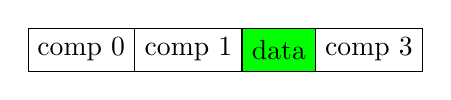
\begin{tikzpicture}[auto]

    \node [instruction-bits-variable,
           rectangle split parts = 4,
           rectangle split part fill={white, white, green, white}] (block0)
    {\nodepart{one}   {comp 0}
     \nodepart{two}   {comp 1}
     \nodepart{three}  {data}
     \nodepart{four}  {comp 3}};

\end{tikzpicture}
\caption {The data is located inside the instruction, hence no further
          addressing is required.}
\label {fig:no-addressing}
\end {figure}

\begin {figure}[H]
\centering
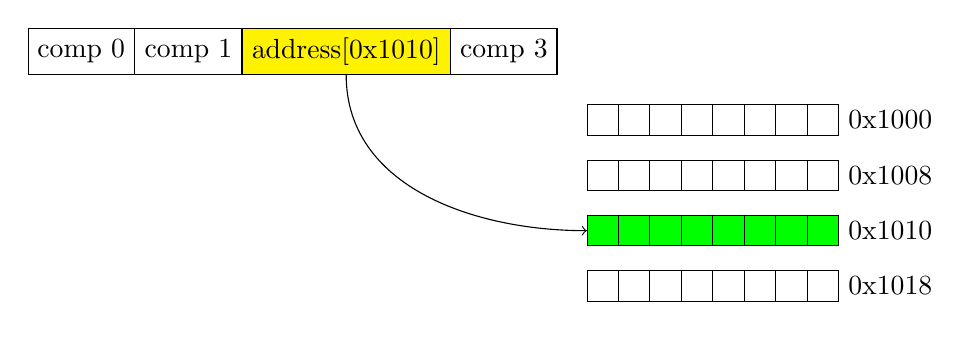
\begin{tikzpicture}[auto]
    \node [instruction-bits-variable,
           rectangle split parts = 8,
           label=east:{0x1000}] (block0) {};

    \node [instruction-bits-variable,
           rectangle split parts = 8,
           label=east:{0x1008},
           node distance = 2em,
           below = of block0.west,
           anchor=west] (block1) {};

    \node [instruction-bits-variable,
           rectangle split parts = 8,
           rectangle split part fill={green},
           label=east:{0x1010},
           node distance = 2em,
           below = of block1.west,
           anchor=west] (block2) {};

    \node [instruction-bits-variable,
           rectangle split parts = 8,
           label=east:{0x1018},
           node distance = 2em,
           below = of block2.west,
           anchor=west] (block3) {};

    \node[fit=(block0)(block1)(block2)(block3)] (mem) {};

    \node [instruction-bits-variable,
           rectangle split parts = 4,
           rectangle split part fill={white, white, yellow, white},
           node distance = 1em,
           above left = of mem] (instr)
    {\nodepart{one}   {comp 0}
     \nodepart{two}   {comp 1}
     \nodepart{three}  {address[0x1010]}
     \nodepart{four}  {comp 3}};

     \draw (instr.three south) edge[out=270,in=180,->] (block2.west) ;

\end{tikzpicture}
\caption {The data is located at the specified memory address. This address
          should be dereferenced to retrieve the data.}
\label {fig:single-level-indirection}
\end {figure}

\subsubsection{Indirect addressing}

There may be one or more stages of indirection:

\begin{itemize}

    \item{Single level indirection - the memory address (or register
        number) of the data is located in a register or another memory
        location as shown in Figure \ref{fig:single-level-indirection}.}

    \item{Multiple level indirection - the data is located at the memory
        location whose address is located at a memory address or
        register. Similarly, the data is located in a register whose
        number is located at a memory address or another register as shown in
        Figure \ref{fig:multi-level-indirection}. Each stage of indirection
        further delays the instruction execution. }

\end{itemize}

\begin {figure}[H]
\centering
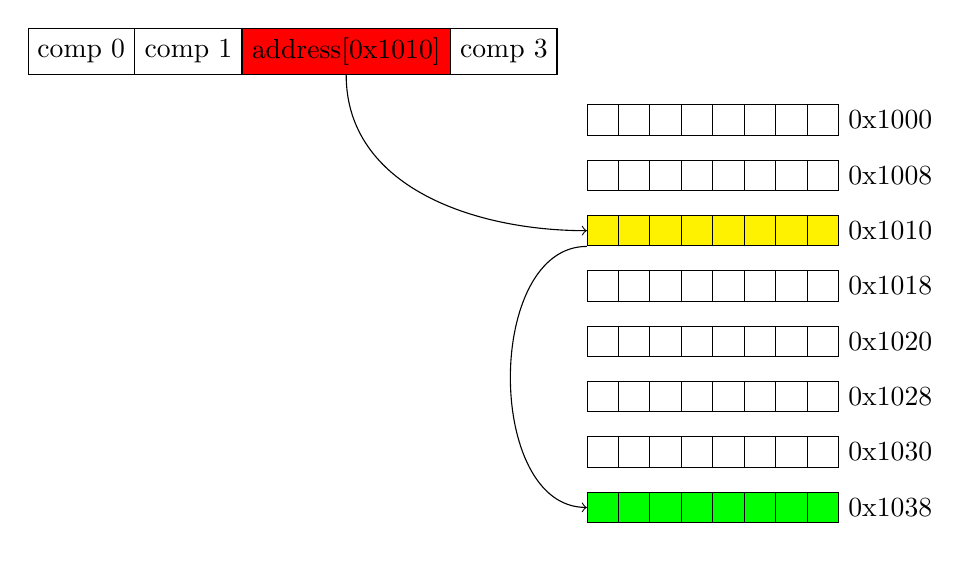
\begin{tikzpicture}[auto]

    \node [instruction-bits-variable,
           rectangle split parts = 8,
           label=east:{0x1000}] (block0) {};

    \node [instruction-bits-variable,
           rectangle split parts = 8,
           label=east:{0x1008},
           node distance = 2em,
           below = of block0.west,
           anchor=west] (block1) {};

    \node [instruction-bits-variable,
           rectangle split parts = 8,
           rectangle split part fill={yellow},
           label=east:{0x1010},
           node distance = 2em,
           below = of block1.west,
           anchor=west] (block2) {};

    \node [instruction-bits-variable,
           rectangle split parts = 8,
           label=east:{0x1018},
           node distance = 2em,
           below = of block2.west,
           anchor=west] (block3) {};

    \node [instruction-bits-variable,
           rectangle split parts = 8,
           label=east:{0x1020},
           node distance = 2em,
           below = of block3.west,
           anchor=west] (block4) {};

    \node [instruction-bits-variable,
           rectangle split parts = 8,
           label=east:{0x1028},
           node distance = 2em,
           below = of block4.west,
           anchor=west] (block5) {};

    \node [instruction-bits-variable,
           rectangle split parts = 8,
           label=east:{0x1030},
           node distance = 2em,
           below = of block5.west,
           anchor=west] (block6) {};

    \node [instruction-bits-variable,
           rectangle split parts = 8,
           rectangle split part fill={green},
           label=east:{0x1038},
           node distance = 2em,
           below = of block6.west,
           anchor=west] (block7) {};

    \node[fit=(block0)
              (block1)
              (block2)
              (block3)
              (block4)
              (block5)
              (block6)
              (block7)] (mem) {};

    \node [instruction-bits-variable,
           rectangle split parts = 4,
           rectangle split part fill={white, white, red, white},
           node distance = 1em,
           above left = of mem] (instr)
    {\nodepart{one}   {comp 0}
     \nodepart{two}   {comp 1}
     \nodepart{three}  {address[0x1010]}
     \nodepart{four}  {comp 3}};

     \draw (instr.three south) edge[out=270,in=180,->] (block2.west) ;
     \draw (block2.south west) edge[out=180,in=180,->] (block7.west) ;

\end{tikzpicture}
\caption {The data is located at the specified memory address in another memory
location. First the address 0x1010 (red) should be dereferenced to obtain a
second address (yellow). The second address should be dereferenced to obtain
the data (green).}
\label {fig:multi-level-indirection}
\end {figure}

The addresses used for indirect addressing can be of 2 types:

\begin{itemize}
    \item{Absolute - the complete address is available. }
    \item{Relative - the relative address to the current instruction pointer is
        available. This is only possible in von Newman architectures as the data
        memory is shared with the instruction memory. This type of addressing
        (compared to absolute addressing) exploits spacial locality as the
        data/instructions surrounding the current instruction are highly likely
        to be cached (though this depends on the caching strategy). }
\end{itemize}

The indirection at each stage may be simple or complex:

\begin{itemize}
    \item{Simple indirection - The address at which the data is located is
        stored in plain format. It can be read and dereferenced directly without
        the need of any additional computation. }
    \item{Complex indirection - The address at which the data is located should
        be calculated to produce a full address. This involves taking a base
        address, and adding a scaled index to it altogether known as SIB (scale,
        index, base) addressing as shown in Equation \ref{eq:SIB}. The scale,
        index and base components can be literals, or the values of some
        registers or memory locations and is hence slower than simple
        indirection.}
\end{itemize}

\begin{equation}
    \label{eq:SIB}
    effective\_address = base + scale * index
\end{equation}

\end{document}
